\documentclass{beamer}
\usetheme{Singapore}

\usepackage{amsmath,amssymb,latexsym}
\usepackage{graphicx}
\usepackage{fancyvrb}
\usepackage{hyperref}

\newcommand{\bi}{\begin{itemize}}
\newcommand{\ii}{\item}
\newcommand{\ei}{\end{itemize}}
\newcommand{\Show}[1]{\psshadowbox{#1}}

\newcommand{\set}[1]{\ensuremath{\left\{ #1 \right\}}}
\newcommand{\nats}{\ensuremath{\mathbb{N}}}
\newcommand{\nni}{\ensuremath{\mathbb{N}^0}}
\newcommand{\ints}{\ensuremath{\mathbb{Z}}}
\newcommand{\power}{\ensuremath{\mathcal{P}}}

\newcommand{\grf}[2]{\centerline{\includegraphics[width=#1\textwidth]{#2}}}
\newcommand{\tw}{\textwidth}
\newcommand{\bc}{\begin{columns}}
\newcommand{\ec}{\end{columns}}
\newcommand{\cc}[1]{\column{#1\textwidth}}

\newcommand{\bfr}[1]{\begin{frame}[fragile]\frametitle{{ #1 }}}
\newcommand{\efr}{\end{frame}}

\newcommand{\cola}[1]{\begin{columns}\begin{column}{#1\textwidth}}
\newcommand{\colb}[1]{\end{column}\begin{column}{#1\textwidth}}
\newcommand{\colc}{\end{column}\end{columns}}

\title{Book of Proof: Fundamentals}

\RecustomVerbatimEnvironment{Verbatim}{Verbatim}{frame=single}

\begin{document}
\begin{frame}
\maketitle

\end{frame}

\bfr{Sets: A mathematical structure}



\begin{align*}
&  \{1,2,3\} \\
&  \set{a,b,c,d} \\
&  \set{cat, dog, pig}\\
&  \set{2,4,6,8,...}\\
  \emptyset &= \{\}\\
  \emptyset &\not= \{\emptyset\}\\
\end{align*}

Note: \set{1,2,3} is not the same as \ensuremath{1,2,3} or \ensuremath{(1,2,3)} or {\em etc.}

\end{frame}

\bfr{Sets have no order or duplicates}
\begin{align*}
  \{1,2,3\}
&= \{2,3,1\}\\
&= \{2,1,3\}\\
  &=  \{1,1,2,2,3,3\} \\
&= \{2,3,3,2,1,1,1,1,2,3,2,2,2,3,1\}\\
\end{align*}


\end{frame}

\bfr{Some important sets}
The integers, the natural numbers, the nonnegative integers
\begin{align*}
  \mathbb{Z} &= \{...,-3,-2,-1,0,1,2,3,4,...\} \\
  \mathbb{N} &= \{1,2,3,4,...\}  \\
  \mathbb{N}^0 &= \{0,1,2,3,4,...\}  \\
\end{align*}

We won't have much use for the real numbers, $\mathbb{R}$.
\end{frame}

\bfr{The size of a finite set}
\begin{align*}
3 &=  |\{a,b,c\}| \\
5 &=  |\{a,b,c,d,e\}| \\
 &=  |\{a,b,c,d,e,a,d,b\}| \\
0 &=  |\emptyset| \\
1 &=  |\{\emptyset\}| \\  
1 &=  |\{\{\emptyset\}\}| \\  
\end{align*}

\end{frame}

\bfr{Membership and subsets}
\begin{align*}
  3 &\in \set{1,2,3,4,5}\\
  3 &\not\in \set{2,4,6,8}\\
  cat &\in \set{cat, dog, pig}\\
  3 &\in \nni\\
  \pi &\not\in \ints\\
  \\
  \set{2,5,8} &\subseteq \set{1,2,3,4,5,6,7,8,9,10}\\
  \set{2,5,8} &\not\subseteq \set{1,2,3,4,5,6,7}\\
  \set{3} &\subseteq \set{1,2,3,4,5}\\
  \set{3} &\not\subseteq \set{2,4,6,8}\\
  \nni &\subseteq \ints \\
  \mathbb{R} &\not\subseteq \nats
  \end{align*}

\end{frame}
\bfr{Set builder notation}
\begin{align*}
  \set{n : \mbox{$n$ is odd and $4\leq n \leq 16$}}
  &= \set{5,7,9,11,13,15}\\
  \set{2n+5 : n\in\set{3,6,7}} &= \set{11,17,19}\\
  \set{2n: n\in\nni} &= \set{0,2,4,6,8,...}\\
  \set{n\in\nats : n < 5} &= \set{1,2,3,4}\\
  \set{3n: n\in\nats \mbox{ and } n < 5} &= \set{3,6,9,12}\\
\end{align*}

\end{frame}

\bfr{Ordered pairs, triples, $n$-tuples}
\begin{align*}
  (2,4) &\not= (4,2)\\
  (2,2) &\not= (2)\\
  (1,2,3) &\not=(3,2,1)\\
  (1,1,2) &\not=(1,2)\\
  (5,3,2,1,6) &\not= (1,2,3,5,6)\\
\end{align*}
\end{frame}

\bfr{Cartesian product}
  
\begin{align*}
A \times B &= \set{(x,y) : x\in A \mbox{ and } y \in B}\\
\set{a,b}\times\set{1,2,3} &= \set{
  (a,1), (a,2), (a,3), (b,1), (b,2), (b,3)}\\
\end{align*}

If $A$ and $B$ are finite sets, then $|A\times B| = |A|\cdot|B|$.
\end{frame}

\bfr{Higher order Cartesian products}
\begin{align*}
  A\times B\times C &= \set{(a,b,c) : a\in A,b\in B, c\in C}\\
  A^n &= A\times A\times A \times... \times A\\
   &= \set{(x_1, x_2, x_3, ..., x_n) : x_1,x_2,x_3,...,x_n\in A}\\
\end{align*}
\end{frame}

\bfr{Power set: the set of all subsets}

\begin{align*}
  \power(\set{a,b,c}) &= \set{\emptyset,\set{a},\set{b},\set{c},
    \set{a,b},\set{a,c},\set{b,c},\set{a,b,c}}
\end{align*}

How many subsets are there?
\end{frame}


\bfr{If $|A| = n$ then $|\power(A)| = 2^n$}

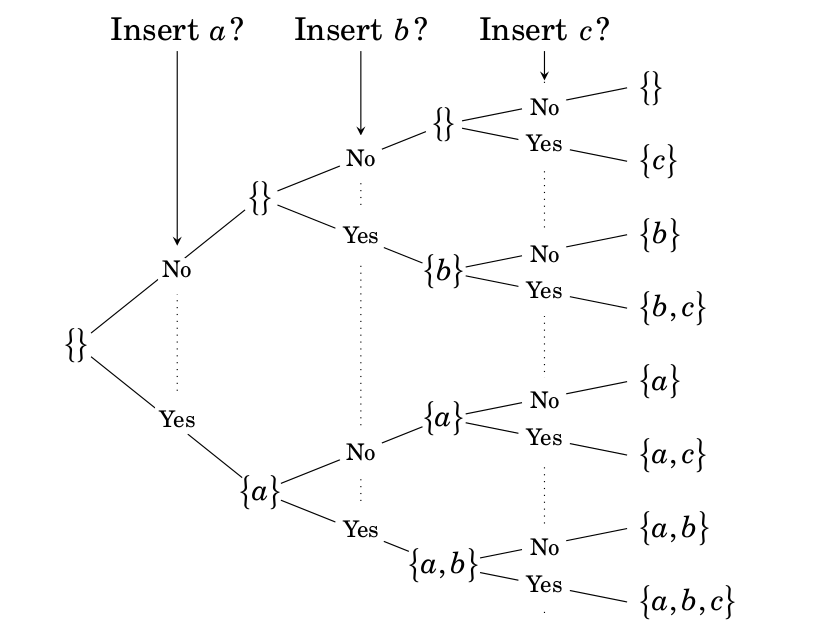
\includegraphics[width=.8\textwidth]{powersettree.png}

\end{frame}


\bfr{Union, Intersection, Difference}
\begin{align*}
  A\cup B &= \set{x : x\in A \mbox{ or } x \in B}\\
  A\cap B &= \set{x : x\in A \mbox{ and } x \in B}\\
  A - B &= \set{x : x\in A \mbox{ and } x \not\in B}\\
  \\
  A &= \set{1,2,3,4,5}\\
  B &= \set{4,5,6,7,8}\\
  A \cup B &= \set{1,2,3,4,5,6,7,8}\\
  A \cap B &= \set{4,5}\\
  A - B &= \set{1,2,3}\\
  \end{align*}

\end{frame}

\bfr{Complement}
\begin{align*}
  \overline{A} &= \set{x : x\not\in A}\\
  \\
  \overline{\set{2,4,6,8,...}} &= \set{1,3,5,7,...}\\
\end{align*}

Usually relative to some implied {\bf universal set} or {\bf universe},
in this case, \nats.

\end{frame}

\bfr{Indexed Sets}
\begin{align*}
  \bigcup_{i=1}^n A_i &= A_1 \cup A_2 \cup A_3 \cup ... \cup A_n\\
  \bigcap_{i=1}^n A_i &= A_1 \cap A_2 \cap A_3 \cap ... \cap A_n\\
\end{align*}
\end{frame}

\bfr{Indexed Sets}
\begin{align*}
  A_i &= \set{ni : n\in\nats}\\
  A_1 &= \set{1,2,3,4,...}\\
  A_2 &= \set{2,4,6,8,...}\\
  A_3 &= \set{3,6,9,12,...}\\
  A_4 &= \set{4,8,12,16,...}\\
      &...\\
  \\
  \bigcup_{i=2}^4 A_i &= \set{2,3,4,6,8,9,10,12,14,15,...}\\
  \bigcap_{i=2}^4 A_i &= \set{12,24,36,48,72,...}\\
\end{align*}
\end{frame}

\bfr{Indexed Sets}
\begin{align*}
\end{align*}
\end{frame}

\end{document}
